% -*- latex -*-
%%%%%%%%%%%%%%%%%%%%%%%%%%%%%%%%%%%%%%%%%%%%%%%%%%%%%%%%%%%%%%%%
%%%%%%%%%%%%%%%%%%%%%%%%%%%%%%%%%%%%%%%%%%%%%%%%%%%%%%%%%%%%%%%%
%%%%
%%%% This text file is part of the source of 
%%%% `Introduction to High-Performance Scientific Computing'
%%%% by Victor Eijkhout, copyright 2012-9
%%%%
%%%% This book is distributed under a Creative Commons Attribution 3.0
%%%% Unported (CC BY 3.0) license and made possible by funding from
%%%% The Saylor Foundation \url{http://www.saylor.org}.
%%%%
%%%%
%%%%%%%%%%%%%%%%%%%%%%%%%%%%%%%%%%%%%%%%%%%%%%%%%%%%%%%%%%%%%%%%
%%%%%%%%%%%%%%%%%%%%%%%%%%%%%%%%%%%%%%%%%%%%%%%%%%%%%%%%%%%%%%%%

\Level 0 {Descent methods}

We consider a multivariate function~$f\colon R^N\rightarrow $ and the
problem of finding the vector~$\bar x$ for which is attains its
minimum. Even for smooth functions we are immediately faced with the
fact that there are local and global minima; for now we satisfy
ourselves with finding a local minimum.

Rather than finding the minimum in one large calculation, we use an
iterative strategy where we start with a point~$\bar x$,
updating it to $\bar x+\bar h$, and repeating this process.
The update vector~$\bar h$ is found through a \indexterm{line search}
strategy:
we settle on a \indexterm{search direction}~$\bar h$,
find a \indexterm{step size}~$\tau$ along that direction, and update
\[ \bar x\leftarrow \bar x+\tau \bar h. \]

\Level 1 {Steepest descent}

Using the multi-dimensional form of the Taylor expansion formula
(section~\ref{app:taylor}) we can write any sufficiently smooth
function as
\[ f(\bar x+\bar h) = f(\bar x) + \bar h^t \nabla f +\cdots. \]
it is not hard to see that choosing $\bar h=-\nabla f$ gives the most
minimization, so we set
\[ x_{\scriptstyle\mathrm{new}}\equiv x-\tau \nabla f. \]
This method is called \indextermdef{gradient descent}
or
\emph{steepest descent}\index{steepest descent|see{gradient descent}}.

For the new function value this gives
\[ f(\bar x - \tau \nabla f ) \approx f(\bar x) - \tau \| \nabla f \|^2 \]
so for $\tau$ small enough this makes the new function value both
positive, and less than~$f(\bar x)$.

The \indexterm{step size} $\tau$ can be computed for quadratic
functions~$f$, and approximated otherwise:
\[ f(\bar x+\tau\bar h) = f(\bar x) + \tau\bar h^t \nabla f +
\frac{\tau^2}2 h^t (\nabla\cdot\nabla f) h +\cdots. \]
Ignoring higher order terms and setting
$\delta f/\delta\tau=0$
gives
\[ \tau = - \bar h^t \nabla f / h^t (\nabla\cdot\nabla f) h. \]

Another strategy for finding a suitable step size is known as
\indextermdef{backtracking}:
\begin{itemize}
\item Start with a default step size, for instance $\tau\equiv1$.
\item Then until $f(\bar x+\tau\bar h)<f(\bar x)$ do
  \[ \tau\leftarrow\tau/2. \]
\end{itemize}

\Level 1 {Stochastic gradient descent}

While the gradient is the optimal search direction in any given step,
overall it need not be the best. For instance, for quadratic problems,
which includes many problems from \acp{PDE}, a~better choice is to
orthogonalize search directions. On the other hand, in \ac{ML}
applications, \indexac{SGD} is a good choice, where the coordinate
directions are used as search directions. In this case
\[ f(x+\tau e_i) = f(x) + \tau \frac{df}{de_i} +
\frac{\tau^2}2 \frac{\delta^2f}{\delta e_i^2} \]
Then:
\[ \tau = - (\nabla f)_i / \frac{ \delta^2 f }{ \delta e_i^2 }. \]

\Level 1 {Code}

\Level 2 {Preliminaries}

We declare a \n{vector} class that is a standard vector, with
operations defined on it such as addition, but also rotation.

There is a derived class \n{unit_vector} that does the obvious.

\Level 2 {Framework}

We start by defining functions as a pure virtual class, meaning that
any function needs to support the methods mentioned here:

\cverbatimsnippet{functiondef}

Using such a function it becomes possible to define various update
steps. For instance, the steepest descent step uses the gradient:

\cverbatimsnippet{steepestdescentstep}

On the other hand, stochastic descent is based on unit vectors:

\cverbatimsnippet{stochasticdescentstep}

\Level 2 {Sanity tests}

Using steepest descent on a circle gives convergence in one step:
%
\snippetwithoutput{descentcircle}{code/minimization}{descentcircle}

On the other hand, steepest descent on an ellipse takes a number of
iterations:
%
\snippetwithoutput{descentellipse}{code/minimization}{descentellipse}

\Level 0 {Newton's method}

\emph{Newton's method}\index{Newton's method|textbf}
%
(or the
\emph{Newton-Raphson method}\index{Newton-Raphson|see{Newton's method}})
%
is an iterative
procedure for finding a \indextermbus{zero}{of a function}, that is, a
value~$x$ for which~$f(x)=0$. It requires knowledge of the derivative~$f'$
of the function, and it can be justified from figures such
as~\ref{fig:newton1d}.

Another justification comes from minimization: if a function~$f$ is
twice differentiable, we can write
\[ f(x+h) = f(x) + h^t\nabla f + \frac12 h^t(\nabla^2f) h \]
and the minimum is attained at
\[ x_{\scriptstyle\mathrm{new}} = x - (\nabla^2f)\inv \nabla f. \]
This equivalent to finding a zero of the gradient:
\[ 0=\nabla f(x+h) = \nabla f(x)+h^t(\nabla^2f(x))h. \]

\begin{exercise}
  Let $f(x_1,x_2) = (10x_1^2+x_2^2)/2 + 5\log(1+e^{-x_1-x_2})$.
  How fast do gradient descent and the Newton's method converge?
  To get insight in their differing behaviors, plot a number of
  iterates against level curves of the function.
\end{exercise}

This exercise gives some idea of that is wrong with gradient descent:
it always steps perpendicular to the current level curve. However, the
minimum does not necessarily lie in that direction.

\begin{figure}[ht]
  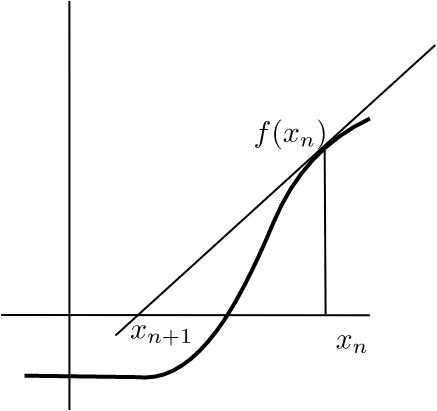
\includegraphics[scale=.3]{newton1d}
  \caption{One step in the one-dimensional Newton method}
  \label{fig:newton1d}
\end{figure}

Iteratively:
\[ x_{n+1} = x_n-f(x_n)/f'(x_n) \]

Without proof we state:
\begin{itemize}
\item The Newton method will converge to the zero if the starting
  point of the iteration is close enough to the zero, and if the
  function is differentiable in the zero.
\item For many functions Newton's method will not converge, but it is
  possible to obtain convergence by introducing damping,
  or doing an inexact update:
  \[ x_{n+1} = x_n-\alpha f(x_n)/f'(x_n) \]
  where $\alpha<1$.
\end{itemize}

\begin{exercise}
  It is possible for Newton's method to be in a cycle. Suppose this is
  a cycle of length two: \[ x_0\rightarrow x_1 \rightarrow x_2=x_0. \]
  If you write out the equations for this cycle you'll find a
  differential equation for~$f$. What is the solution? Why doesn't the
  Newton method converge for this function?
\end{exercise}

In multiple dimensions, that is, with a function
$f\colon\mathbb{R}^N\rightarrow\mathbb{R}$
Newton's method becomes an iterated
\emph{linear system solution}%
\index{Newton's method!and linear system solving|see{linear system, solving}}
\index{linear system!solving!in Newton's method}:
\[ \bar x_{n+1} = \bar x_n-F(\bar x_n)\inv f(\bar x_n) \]
where $F$ is the \indexterm{Jacobian} of~$f$.

Since Newton's method is an iterative process we do not need the
solution of this linear system to full accuracy, so inexact solutions,
for instance through
\emph{iterative solution}\index{linear system!iterative solution},
is often feasible.

\Level 1 {Inexact Newton's method}

There is a variety of reasons why Newton's method would not converge.
(In fact, plotting the regions from where it does converge will, for
suitable functions, give nice \indexterm{fractals}.)
For this reason, in practice an
\indextermsub{inexact}{Newton's method} is used. The inexactness comes
in two ways:
\begin{itemize}
\item Instead of the `optimal' step length we use a fraction. This is
  often chosen through `backtracking', and a choice is adopted for
  which at least some decrease in function value is observed.
\item Instead of the inverse of the Jacobian we use an approximation
  of that operator. For instance, we could compute the Jacobian (often
  an expensive process) and then use it for multiple Newton steps.
\end{itemize}
A combination of these techniques can be shown to give guaranteed
converence~\cite{zhwa94}.
